\documentclass{article}

\usepackage[T1]{fontenc}
\usepackage[utf8]{inputenc}
%\usepackage[french]{babel}
\usepackage{graphicx}
\usepackage{hyperref}
\usepackage{lmodern}
\usepackage{amsmath}
\usepackage{amsthm}
\usepackage{listings}
\usepackage{enumerate}
\usepackage{amssymb}
\usepackage{amsfonts}
\usepackage{float}

\usepackage[a4paper]{geometry}

\author{Latrille Thibault, Laurent Duret, Nicolas Lartillot}
\title{The red queen dynamic in the kingdom of recombination.}  

\sloppy 

\begin{document}

\maketitle 

\newcommand{\Ne}{N_\mathrm{e}}

%\tableofcontents             

\section{Abstract}

In humans and many other species, recombination events cluster into narrow hotspots within the genome. Given the vital role recombination plays in meiosis, we might expect that the positions of these hotspots would be tightly conserved over evolutionary time. However, there is now strong evidence that hotspots of meiotic recombination in humans are transient features of the genome. For example, hotspot locations are not shared between human and chimpanzee. Biased gene conversion in favor of alleles that locally disrupt hotspots is a possible explanation of the short lifespan of hotspots.

Remarkably, Prdm9 has been proposed to be a key determinant of the positioning of recombination hotspots during meiosis, and the most rapidly evolving gene in human. Prdm9 genes often exhibit substantial variation in their numbers of encoded zincfingers, not only between closely related species but also among individuals of a species.

Here, we propose a population genetic model which exhibits hotspots transience while reflecting the PRDM9 features, resulting in a intragenomic red queen dynamic. Our model account for empirical observations regarding the molecular mechanisms of recombination hotspots and the nonrandom targeting of the recombination by PRDM9. We further investigate and compare to known data the diversity of PRDM9, the hotspots turnover and the genome wide disruption of hotspots.


\section{Introduction}

PRDM9 is a meiosis-specific histone methyltransferase with a tandem-repeat zinc finger (ZnF) domain encoded by a mini-satellite-like sequence. The ZnF domain is polymorphic in repeat number and type, and appears to be directly responsible for activating recombination hotspots by binding to hotspot-associated sequence motifs in both humans and mice.

Hotspots evolve rapidly, as shown by the totally different fine-scale recombination landscapes of humans and chimpanzees.
Turnover might be driven by the tendency of hotspots to self-destruct through the systematic over-transmission of variants within hotspots that down-regulate recombination initiation, leading to hotspot depletion and consequent 
selection in favour of PRDM9 variants that activate new sets of hotspots.

We are interested in a mathematical modelling of the turnover of PRDM9 variants and the associated recombination hotspots.

	\begin{figure}[H]
	  \centering
       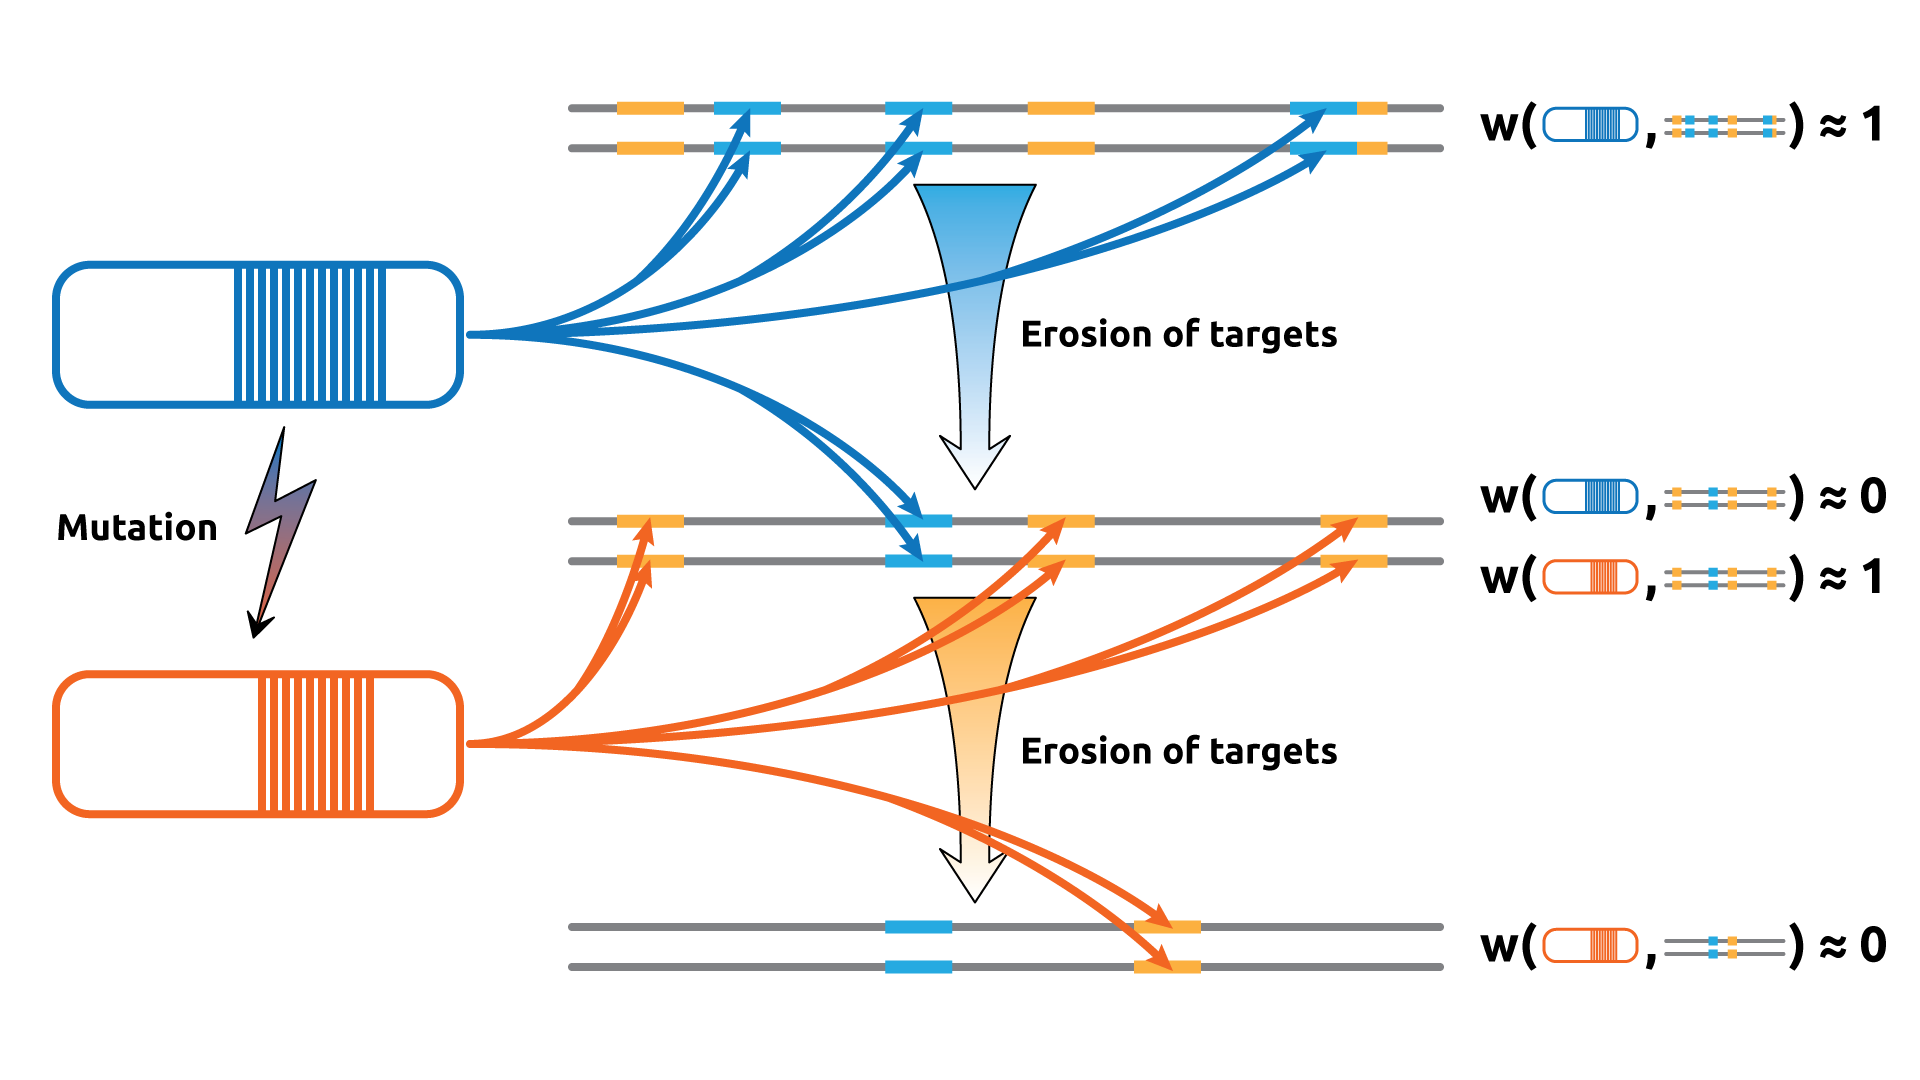
\includegraphics[width=12.0cm]{Images/red-queen.png}\\
		\caption{ \textbf{PRDM9 dynamic}. 
		\label{fig:redqueen}}
	\end{figure}
	
\section{Population genetic model of the red queen}


The population is composed of $\Ne$ diploid individuals, kept constant over time.


The locus PRDM9 mutates at constant rate $u$ per generation per locus and each new variant binds a new sets of sequence targets. Thus $u$ can be understood as a functional mutation rate, with each mutation producing a new PRDM9 variant with new hotspots.


We consider that PRDM9 is binding it's target in *trans*, meaning there is no linkage between the locus of PRDM9 and any of the target. The sequence targets of PRDM9 mutates at constant rate $v$ per generation. The sequence targets recombine at constant rate $r_0$ per generation. The recombination at the sequence target is favoured by the binding of PRDM9.


At each generation, $K$ is the number of PRDM9 variants in the population. $\forall i \in \{ 1, \, \dots, \, K \}$, $n_i$ is the number of $i^{th}$ PRDM9 variant in the population. Consequently, $x_i = n_i / 2 \Ne$ is the frequency of the $i^{th}$ PRDM9 variant.


For each variant, $L_i$ is the overall erosion of the sequence targets, with $L_i=1$ meaning no erosion and $L_i=0$ meaning totally eroded. $\overline{\omega_i}$ is fitness of this variant. At the population level, $\overline{\omega}=\sum_{i} x_i \overline{\omega_i}$ is the mean fitness.

We propose $\overline{\omega_i}=\sum_j x_j f \left( \tfrac{L_i + L_j}{2} \right)$, for any function $f\colon [0,1] \rightarrow \mathbb{R}^+$. Meaning the fitness of variant $i$ is the sum over the probabilities that the second variant is $j$ (diploid individuals) time a function of the mean erosion between variant $i$ and $j$. Thus we assume the variants interact linearly.


\section{Discret and stochastic implementation of the model} 

We derived a mathematic population genetic model, implemented numerically by monte carlo simulations in Python, the code is hosted [**here**](https://github.com/ThibaultLatrille/RedQueen).

For each new generation, the simulation is decomposed in three steps, computed in the following order: 

1. Mutation and creation of new variants of PRDM9
2. Erosion of the recombination hotspots
3. Drift and selection

\subsection{Mutation and creation of new variants of PRDM9} 

Per locus, PRDM9 mutates at constant rate $u$, and we have $2 \Ne$ loci in the population. Thus the number of new variants is Poission distributed with mean $2 \Ne u$. the new variants are introduced in the population at a frequency $1 / 2 \Ne$

\begin{equation}
  K(t+1) - K(t) \sim \operatorname{Pois} \left(2 \Ne u \right)
\end{equation}


\subsection{Erosion of the recombination hotspots} 

PRDM9 activates it's targets in *trans*. The number of new mutation occuring in the population at the targets is $2 \Ne v$, each of them are driven by a selection coefficient $2 r _0  x_i$, where $x_i$ is the probabity of activation by the variant $i$.
Since the strenght of erosion is proportionnal to the targets being not eroded, we model the erosion as an exponential decay.

\begin{equation}
  \begin{aligned}
 L_i (t+1) &=  L_i (t)\operatorname{exp} \left( - 2 \Ne v
 \dfrac{1 - \operatorname{e}^{-2 r _0  x_i}}{1 - \operatorname{e}^{-4 \Ne r _0  x_i}} \right)  \\
 &\simeq
    L_i (t)\operatorname{exp} \left( - 4 \Ne v
 r _0  x_i \right), \;
 \forall i \in \{ 1, \, \dots, \, K \} \\ \\
 \end{aligned}
\end{equation}


\subsection{Drift and selection} 

The new generation of $2 \Ne$ PRDM9 alleles is drawn from a multinomial distribution, generating a drift. The probability of drawing variant $i$ is equal to it's frequency $x_i$ time it's relative fitness  $\tfrac{\overline{\omega_i}}{\overline{\omega}}$. The probabilities sum to $1$ by definition of $\overline{\omega}$.

\begin{equation}
  \left(
  n_1(t+1), \,
  \dots, \,
  n_i(t+1), \,
  \dots, \,
  n_{K(t)}(t+1)
  \right)
  \sim \operatorname{Multinomial} \left(2 \Ne, \,
  \dfrac{x_1  \overline{\omega_1}}{\overline{\omega}}, \,
  \dots, \,
  \dfrac{x_i  \overline{\omega_i}}{\overline{\omega}}, \,
  \dots, \,
  \dfrac{x_{K(t)} \overline{\omega_{K(t)}}}{\overline{\omega}}
  \right)
\end{equation}


\section{Approximation for the fitness function}
Let us denote $\overline{L}=\sum_i x_i L_i$.

One can use a Taylor approximation to linearize the fitness function around $\overline{L}$.  

\begin{equation}
  \begin{aligned}
    \overline{\omega_i} - f(\overline{L}) &=
    \sum_j x_j f \left( \tfrac{L_i + L_j}{2} \right) - \sum_j x_j f(\overline{L}) \\
    &=
    \sum_j x_j  \left[ f \left( \tfrac{L_i + L_j}{2} \right) - f(\overline{L}) \right] \\
    &\simeq
    \sum_j x_j  f'(\overline{L}) \left( \tfrac{L_i + L_j}{2} - \overline{L} \right) \\
    &\simeq
     f'(\overline{L}) \left( \tfrac{L_i + \sum_j x_j L_j}{2} - \overline{L} \right) \\
     &\simeq
     f'(\overline{L}) \left( \tfrac{L_i - \overline{L}}{2}\right) \\
  \end{aligned}
\end{equation}

Consequently $\overline{\omega} = f(\overline{L})$. *Proof*,

\begin{equation}
  \begin{aligned}
    f(\overline{L}) &= \sum_i x_i f(\overline{L}) \\
    &\simeq \sum_i x_i \left[ \overline{\omega_i} - f'(\overline{L}) \left( \tfrac{L_i - \overline{L}}{2}\right) \right] \\
    &\simeq
    \sum_i x_i \sum_i x_i \overline{\omega_i} - \sum_i x_i f'(\overline{L}) \left( \tfrac{L_i - \overline{L}}{2}\right) \\
    &\simeq
     \overline{\omega} - f'(\overline{L}) \sum_i x_i \left( \tfrac{L_i - \overline{L}}{2}\right) \\
    &\simeq
     \overline{\omega}
  \end{aligned}
\end{equation}

And the selection coefficient $s_i$ for the variant $i$ can be easily computed  

\begin{equation}
    s_i = \dfrac{\overline{\omega_i} - \overline{\omega}}{\overline{\omega}}
    \simeq  \dfrac{f'(\overline{L})}{f(\overline{L})} \left[ \tfrac{L_i - \overline{L}}{2} \right]
\end{equation}

Thus the probability of drawing variant $i$ in the multinomial distribution is given by 
\begin{equation}
    x_i \dfrac{\overline{\omega_i}}{\overline{\omega}} = 
     x_i (1 + s_i) =  x_i \left(1 +  \dfrac{f'(\overline{L})}{f(\overline{L})} \left[ \tfrac{L_i - \overline{L}}{2} \right] \right)
\end{equation}

\section{Continuous time derivation of the model}
Assuming there is no mutation of PRDM9, and by discarding the drift altogether, we derive a close set of differential equations for the frequencies of PRDM9 and the erosion of the targets.

\begin{equation}
  \left\{
      \begin{aligned}
        \mathrm{\Delta}L_i &= 
        - 4 \Ne v r _0  x_i L_i \mathrm{\Delta}t, \;
             \forall i \in \{ 1, \, \dots, \, K \} \\
        \mathrm{\Delta}x_i &= \dfrac{f'(\overline{L})}{f(\overline{L})} \left[ \tfrac{L_i - \overline{L}}{2} \right]x_i  \mathrm{\Delta}t , \;
         \forall i \in \{ 1, \, \dots, \, K \}\\
      \end{aligned}
    \right.
 \Rightarrow
  \left\{
      \begin{aligned}
        \dfrac{\mathrm{d}L_i}{\mathrm{d}t} &= 
        - \rho  x_i L_i, \;
             \forall i \in \{ 1, \, \dots, \, K \} \\
        \dfrac{\mathrm{d}x_i}{\mathrm{d}t} &= \dfrac{f'(\overline{L})}{f(\overline{L})} \left[ \tfrac{L_i - \overline{L}}{2} \right]x_i , \;
         \forall i \in \{ 1, \, \dots, \, K \}\\
      \end{aligned}
    \right.
\end{equation}

with $\rho = 4 \Ne v r _0$

\section{Dynamic of the mean erosion}
We denote $\overline{x^{j} L^{k}}=\sum_i x_i^{j} L_i^{k} x_i =\sum_i x_i^{j+1} L_i^{k}$

\subsection{Differential equation of the mean erosion}
As before, let $\overline{L}=\sum_i x_i L_i$ be the mean erosion of the hotspots.

\begin{equation}
  \begin{aligned}
    \dfrac{\mathrm{d} \overline{L} }{\mathrm{d}t} &=
    \sum_i L_i \dfrac{\mathrm{d}x_i}{\mathrm{d}t} +  \sum_i x_i \dfrac{\mathrm{d}L_i}{\mathrm{d}t} \\
    &=
    \dfrac{f'(\overline{L})}{2 f(\overline{L})} \sum_i (L_i - \overline{L}) (L_i - \overline{L}) x_i - \rho \sum_i L_i x_i^2\\
    &=
    \dfrac{f'(\overline{L})}{2 f(\overline{L})} (\overline{L^2} - \overline{L}^2) - \rho \overline{L X}\\
  \end{aligned}
\end{equation}

The first term of the equation is the same sign of $f'(\overline{L})$. If positive it means the less eroded variants will increase in frequency because they are better fit, increasing $\overline{L}$. The second term is always negative, due to the overall erosion of all targets.

\subsection{Adding mutation of PRDM9}

One can add an additional term for mutations of PRDM9 as follows. Variants mutate at a rate $2 \Ne u$, and a the erosion of a new variant is $1$, being previously $\overline{L}$ on average. Taking altogether, $\overline{L}$ increase at a rate  $2 \Ne u (1 - \overline{L})$

\begin{equation}
  \begin{aligned}
    \dfrac{\mathrm{d} \overline{L} }{\mathrm{d}t} &=
    \dfrac{f'(\overline{L})}{f(\overline{L})} (\overline{L^2} - \overline{L}^2) - \rho \overline{L X} + 2 \Ne u (1 - \overline{L})\\
  \end{aligned}
\end{equation}

\subsection{Landscape of erosion}

\begin{equation}
  \begin{aligned}
    V &=  \sum_i L_i^2 x_i  -  \left( \sum_i L_i x_i \right)^2 \\
    &=
    \overline{L^2} - \overline{L}^2 \\
  \end{aligned}
\end{equation}

\section{Dynamic for the PRDM9 diversity}

\subsection{Diversity measures}
Diversity can be defined in several ways; for example the richness $K(t)$, defined above as the number of variants, is a measure of PRDM9 diversity. One shortcoming for $K(t)$ is that it gives equal weight to all variants, regardless of their frequencies in the population. 

An other measure of diversity is the shannon entropy, $\mathrm{e}^{ - \sum_i x_i \mathrm{log}(x_i)}$. 

\subsection{The simpson entropy}
We focus on the simpson entropy $R$. It equals $K(t)$ if all the variants have equal weights and is close to $1$ if only one variant is high frequency and the other are low frequencies.

\begin{equation}
  \begin{aligned}
     R &= \left( \sum_i x_i^2  \right)^{-1} = \dfrac{1}{\overline{X}}
  \end{aligned}
\end{equation}

\subsection{Differential equation for the simpson entropy}
\begin{equation}
  \begin{aligned}
    \dfrac{\mathrm{d} R }{\mathrm{d}t} &=
    - \dfrac{\mathrm{d} \left( \sum_i x_i^2  \right)}{\mathrm{d}t} \left( \sum_j x_j^2  \right)^{-2} \\
    &=
   - 2  \sum_i x_i \dfrac{\mathrm{d} x_i }{\mathrm{d}t} \left( \sum_j x_j^2  \right)^{-2} \\
    &=
    - 2  \sum_i x_i \dfrac{f'(\overline{L})}{f(\overline{L})} \left[ \tfrac{L_i - \overline{L}}{2} \right]x_i \left( \sum_j x_j^2  \right)^{-2} \\
    &=
    - \dfrac{f'(\overline{L})}{f(\overline{L})} \sum_i (L_i - \overline{L})  x_i^2 \left( \sum_j x_j^2  \right)^{-2} \\
     \\
      &=
     \dfrac{f'(\overline{L})}{f(\overline{L})} \left[ \dfrac{\overline{L} \overline{X} - \overline{L X}}{ \overline{X} ^{2}} \right] \\
     &=
     R^2 \dfrac{f'(\overline{L})}{f(\overline{L})} \left[ \overline{L} \overline{X} - \overline{L X} \right] \\
  \end{aligned}
\end{equation}


\section{Trajectory for a single allele}

We set $\overline{L}$ as a fixed parameter, and study closely the trajectory of a single allele.


\subsection{Differential equations}

\begin{equation}
  \left\{
      \begin{aligned}
          \dfrac{\mathrm{d}x}{\mathrm{d}t} &= \dfrac{f'(\overline{L})}{2 f(\overline{L})} \left( l - \overline{L} \right) x \\
        \dfrac{\mathrm{d}l}{\mathrm{d}t} &= 
        - \rho x l \\
      \end{aligned}
    \right.
 \Rightarrow
  \left\{
      \begin{aligned}
          \dfrac{\mathrm{d}x}{\mathrm{d}l} &= \dfrac{f'(\overline{L})}{2 \rho f(\overline{L})}\left( \dfrac{\overline{L}}{l} -1 \right) \\
        \dfrac{\mathrm{d}l}{\mathrm{d}t} &= 
        - \rho x l \\
      \end{aligned}
    \right.
 \Rightarrow
  \left\{
      \begin{aligned}
          x(l) &=\dfrac{f'(\overline{L})}{2 \rho f(\overline{L})} (1-l + \overline{L} \mathrm{log}(l)) + x_{\mathrm{initial}} \\
        \dfrac{\mathrm{d}l}{\mathrm{d}t} &= 
         \dfrac{f'(\overline{L})}{2 f(\overline{L})} [ l-1- \overline{L} \mathrm{log}(l)]l  - \rho x_{\mathrm{initial}} l \\
      \end{aligned}
    \right.
\end{equation}

We get a close solution for the frequency $x$ as a function of $l$. But we couldn't get a close form for both $x$ and $l$ as a function of $t$.


\subsection{Chart}
	\begin{figure}[H]
	  \centering
       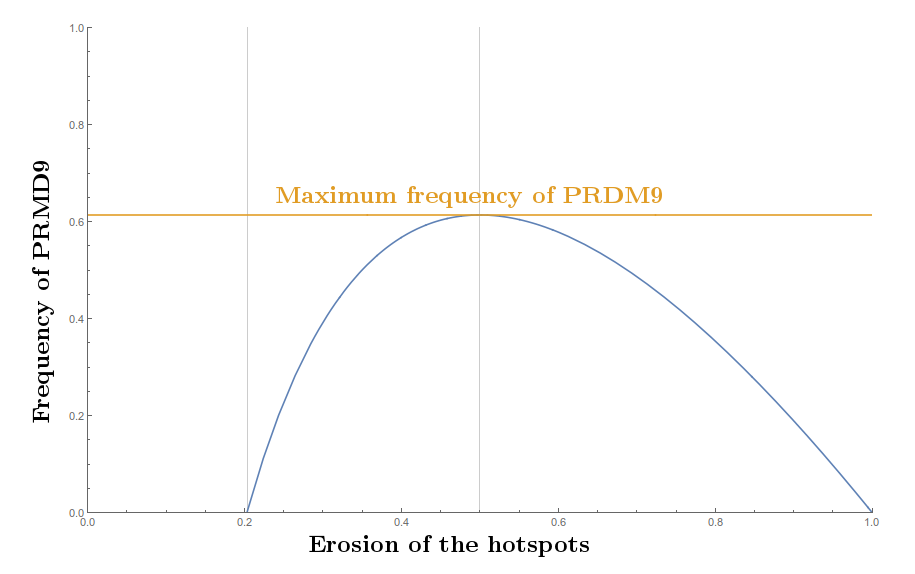
\includegraphics[width=9.0cm]{Images/single-allele.png}\\
		\caption{ \textbf{A hypothetical abundance phylogenetic tree}. 
		\label{fig:singleallele}
		Left panel:  
$x(l)$ as a function of $l$ in solid blue.   
$l.x(l)$ as a function of $l$ in solid yellow.  
$L_{max}$ in green. 
Rigth panel:  
$x(t)$ as a function of $t$ in solid blue.   
$l(t)$ as a function of $t$ in solid green.  
$L_{max}$ in red. 
parameters: $\overline{L} = 0.5$; $\rho = 1$; $\dfrac{f'(\overline{L})}{2 f(\overline{L})} = 4$;}
	\end{figure}
\subsection{Erosion maximum}

\begin{equation}
  \begin{aligned}
    0 &=\dfrac{f'(\overline{L})}{2 \rho f(\overline{L})} (1-l_{\infty} + \overline{L} \mathrm{log}(l_{\infty})) + x_{\mathrm{initial}}\\
       \iff   l_{\infty} &\simeq - \overline{L} \mathrm{W} \left(\dfrac{ - \mathrm{e}^{- 1 / \overline{L}}}{\overline{L}}  \right)
  \end{aligned}
\end{equation}

Where $W$ is the Lambert $W$ function defined such that $W(z)e^{W(z)}=z$
\subsection{Tilling argument}

Using a tilling argument, if the new alleles settle in the population at constant rate, one can change their rate of arrival.
\begin{equation}
  \begin{aligned}
    \overline{x^{j} L^{k}} &= \sum_i x_i^{j+1} L_i^{k} \\
    &= \dfrac{ \int_{0}^{\infty} x(t)^{j+1} l(t)^{k} \mathrm{d} t }{ \int_{0}^{\infty} x(t) \mathrm{d} t }
    \\
    &= \dfrac{ \int_{1}^{l_{\infty}} x(l)^{j} l^{k-1} \mathrm{d} l  }{ \int_{1}^{l_{\infty}} l^{-1} \mathrm{d} l }
    \\
    &= \dfrac{ \int_{1}^{l_{\infty}} \left( \dfrac{f'(\overline{L})}{2 \rho f(\overline{L})} (1-l + \overline{L} \mathrm{log}(l)) + x_{\mathrm{initial}}  \right)^{j} l^{k-1} \mathrm{d} l  }{ \int_{1}^{l_{\infty}} l^{-1} \mathrm{d} l }
    \\
  \end{aligned}
\end{equation}

In particular, we get the simpson diversity R,

\begin{equation}
  \begin{aligned}
    R &= \overline{x}^{-1} \\
    &=  \dfrac{ \int_{1}^{l_{\infty}} l^{-1} \mathrm{d} l }{ \int_{1}^{l_{\infty}} \left( \dfrac{f'(\overline{L})}{2 \rho f(\overline{L})} (1-l + \overline{L} \ln(l)) + x_{\mathrm{initial}}  \right) l^{-1} \mathrm{d} l } 
    \\
    &= \dfrac{4 \rho f(\overline{L})}{f'(\overline{L})\left[ 1 + l_{\infty} - 2 \overline{L}  \right]} 
    \\
  \end{aligned}
\end{equation}

Also, we get the landscape erosion V,

\begin{equation}
  \begin{aligned}
    V &=  \overline{L^2} - \overline{L}^2 \\
    &= \dfrac{ \int_{1}^{l_{\infty}} l \mathrm{d} l  }{ \int_{1}^{l_{\infty}} l^{-1} \mathrm{d} l } - \left( \dfrac{ \int_{1}^{l_{\infty}} \mathrm{d} l  }{ \int_{1}^{l_{\infty}} l^{-1} \mathrm{d} l } \right)^2
    \\
    &= \frac{\overline{L}}{2}  \left(1 + l_{\infty}\right) - \overline{L}^2
    \\
    &= \frac{\overline{L}}{2}  \left(1 + l_{\infty} - 2 \overline{L}\right)
    \\
  \end{aligned}
\end{equation}


\section{Estimation of $\overline{L}$}
\subsection{Estimation of interval}

\begin{equation}
  \begin{aligned}
    \tau_{\mathrm{inter}}^1 &= \int_{1}^{l_{\infty}} x \mathrm{d} t = \dfrac{1 - l_{\infty}}{\overline{L} \rho} \\
    \tau_{\mathrm{inter}}^2 &= \dfrac{1}{2 \Ne v \dfrac{f'(\overline{L})}{f(\overline{L})} (1-\overline{L})  }
  \end{aligned}
\end{equation}

\begin{equation}
  \begin{aligned}
    \tau_{\mathrm{inter}}^1 = \tau_{\mathrm{inter}}^2 \Rightarrow 
    \dfrac{f'(\overline{L})}{f(\overline{L})} \dfrac{(1- \overline{L})(1- l_{\infty})}{\overline{L}} = \dfrac{v r_o}{2 u}
  \end{aligned}
\end{equation}

\section{Longevity of PRDM9}
\subsection{For a single allele}

\begin{equation}
  \begin{aligned}
    \dfrac{1}{\overline{L}} \left( \dfrac{\mathrm{d}l}{\mathrm{d}t} \right)_{\overline{L}}
    &= \dfrac{f'(\overline{L})}{2 f(\overline{L})} [ \overline{L}-1 + \overline{L} \ln(\overline{L})] \\
    &\simeq \dfrac{\alpha}{2 \overline{L}}[\overline{L}-1 + \overline{L} \ln(\overline{L})] = \dfrac{1}{\tau} \\
  \end{aligned} \\
  \Rightarrow \tau \simeq \dfrac{2 \overline{L}}{\alpha[\overline{L}-1 + \overline{L} \ln(\overline{L})]}
\end{equation}

\bibliographystyle{plain}

\end{document}





